\section{State Of The Art Analysis}\label{sec:state-of-the-art-analysis}
This section will discuss the state of the art of technologies already used in amusement parks around the world.
It will also focus on those used, or that have been used in the past, in the park Mirabilandia in Italy.

Firstly, since an incarnation of a Micro City as an amusement park has the crucial ``queue'' concept, we searched for ``smart''
and innovative solutions to manage that.
Another important point in a Micro City is that the system should be able to send notifications based on the location of
the people at a certain time.
Another is the personalization of the experience.

\subsection{Virtual Queueing}\label{subsec:virtual-queueing}

\subsection{Accesso Technology Group}\label{subsec:accesso-technology-group}
Accesso Technology Group\footnote{\url{https://www.accesso.com/}} (formerly Lo-Q) is an English company that provides
devices and mobile apps for virtual queueing to several clients, including theme parks like the ``Six Flags'' corporation in the US
and ``LEGOLAND Windsor Resort'' in the UK\@.

Their products for virtual queueing are \textit{Qsmart} and \textit{Prism}\footnote{\url{https://www.accesso.com/solutions/virtual-queuing}}
that nowadays replace the devices \textit{Qbot} and \textit{Qband}.
With Qsmart people can access the virtual queueing services directly from their smartphones whereas Prism is a ``smartwatch-like''
wearable.
As can be observed in Figure\ref{fig:prismart}, the main functionalities of both QSmart and Prism are:

\begin{figure}[H]
    \centering
    \begin{subfigure}[b]{0.85\textwidth}
        \centering
        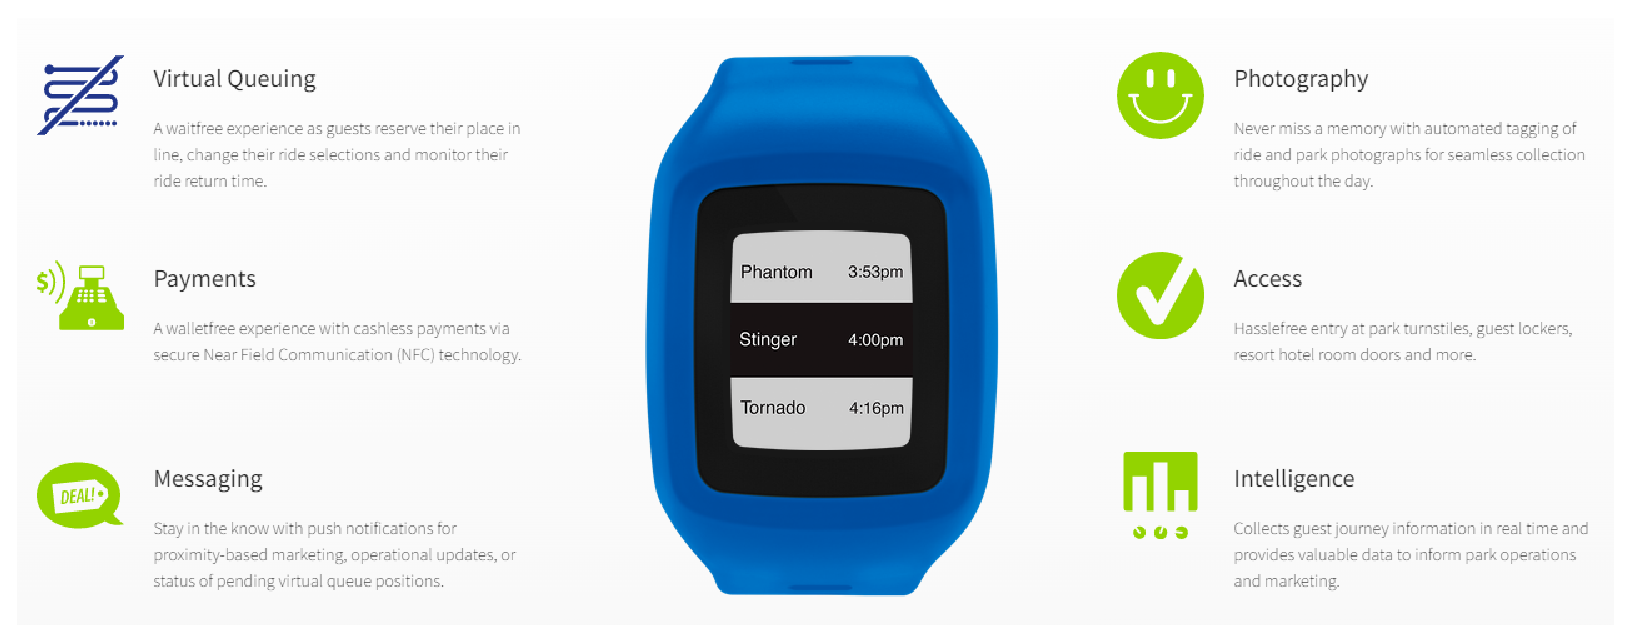
\includegraphics[width=\textwidth]{img/prism}
        \caption{Prism main functionalities}
        \label{fig:prism}
    \end{subfigure}
    \hfill
    \begin{subfigure}[b]{0.85\textwidth}
        \centering
        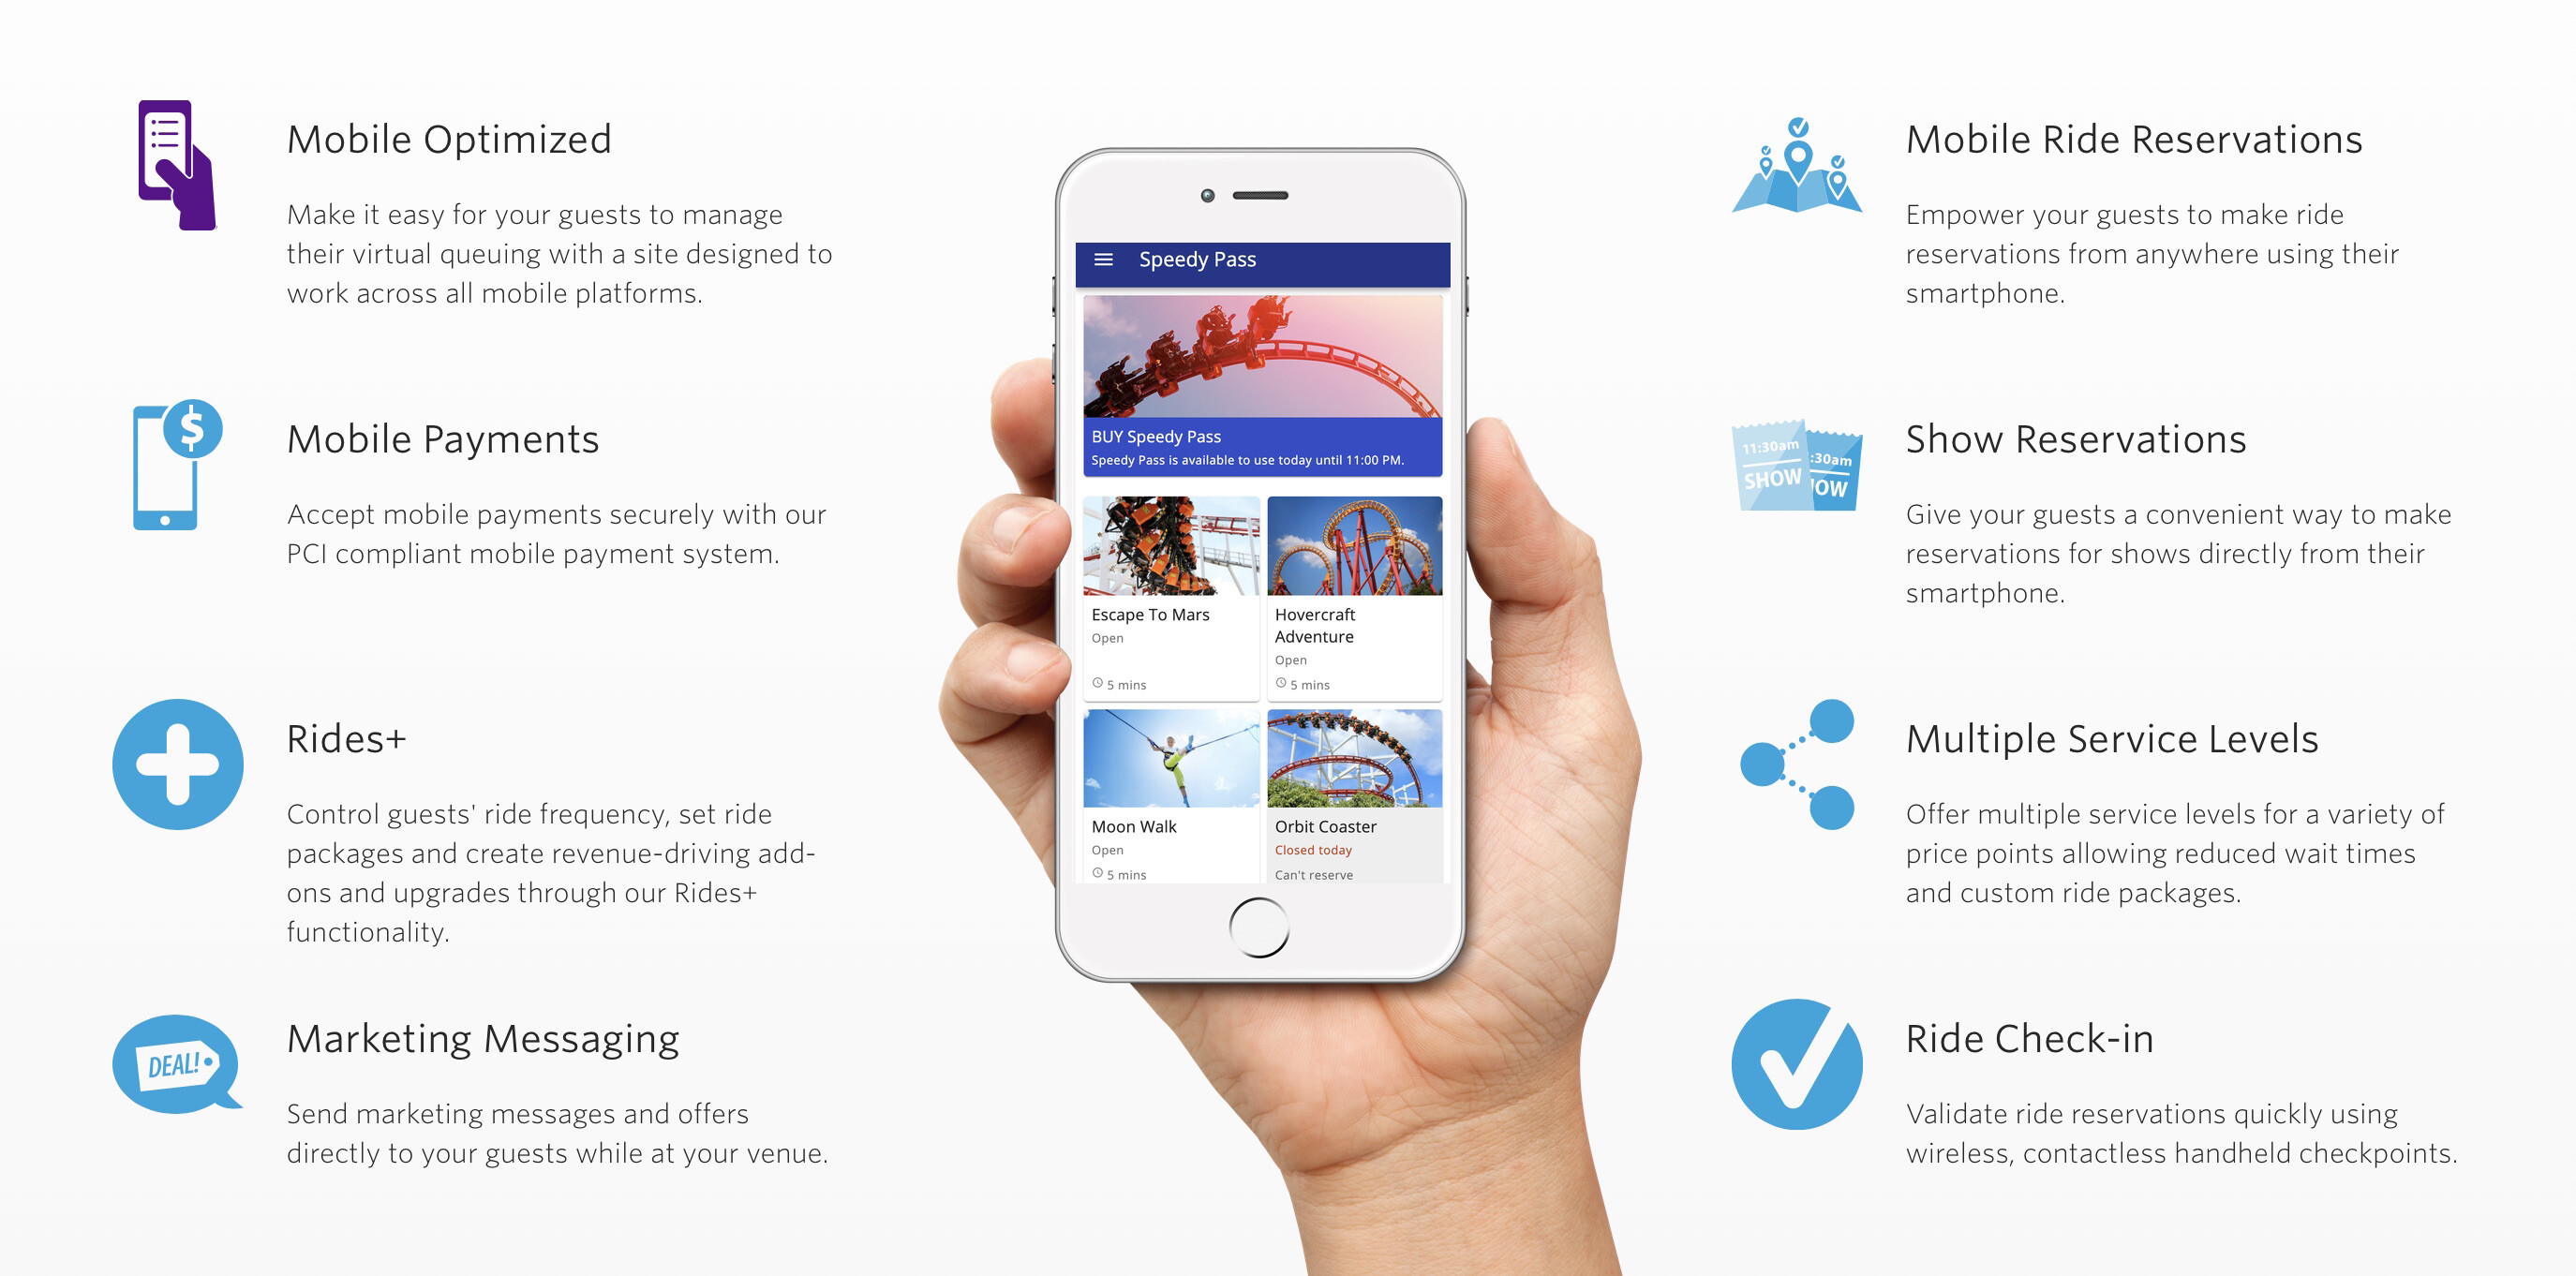
\includegraphics[width=\textwidth]{img/qsmart}
        \caption{Qsmart main functionalities}
        \label{fig:qsmart}
    \end{subfigure}
    \caption{Accesso's products for virtual queueing}
    \label{fig:prismart}
\end{figure}

Both Qsmart and Prism interact with the Virtual Queue Management System, where customers can consult
analytics and performance data as well as control in real-time the virtual queueing solution.
However, there isn't much information about this product on the company website.

Prism uses three technologies for communications:
\begin{itemize}
    \item Bluetooth Low Energy Communication:
    \item Near Field Communication (NFC):
    \item Sub-GHz Two-Way Radio:
\end{itemize}

They provided their Q-Bot device also to Mirabilandia in 2009 but is no longer used nowadays.

\subsubsection{Accesso's Virtual Queueing}
Their technology is patented.

\subsection{Mirabilandia App}\label{subsec:mirabilandia-app}
- fornisce già percorsi specifici per chi è interessato a giochi adrenalinici, per bambini ecc.

\subsection{Mirabilandia - V Pass}\label{subsec:mirabilandia-v-pass}
differenza V Pass e Flash Pass.
il Disney FastPass

\subsection{Legoland Windsor - Reserve and Ride}\label{subsec:legoland-windsor---reserve-and-ride}

